\documentclass[a4paper, 12pt]{article}%тип документа

%отступы
\usepackage[left=2cm,right=2cm,top=2cm,bottom=3cm,bindingoffset=0cm]{geometry}

%Русский язык
\usepackage[T2A]{fontenc} %кодировка
\usepackage[utf8]{inputenc} %кодировка исходного кода
\usepackage[english,russian]{babel} %локализация и переносы

%Вставка картинок
\usepackage{wrapfig}
\usepackage{graphicx}
\graphicspath{{pictures/}}
\DeclareGraphicsExtensions{.pdf,.png,.jpg}

%Графики
\usepackage{multirow}
\usepackage{pgfplots}
\pgfplotsset{compat=1.9}

%Математика
\usepackage{amsmath, amsfonts, amssymb, amsthm, mathtools}

%Заголовок
\author{Сифат Мд Абдуллах Ал Хасиб \\
Факультет физической и квантовой электроники \\
Группа Б04-105}
\title{\textbf{Лаборатория Работа 1.3.3 \\ 
Определение вязкости вязкости воздуха по скорости течения через тонкие трубки}}
\begin{document}
\maketitle
\section{Введение}\textbf{Цель работы}: Экспериментально исследовать свойства течения газов по тонким труб-кам при различных числах Рейнольдса; выявить область применимости закона Пуа-зейля и с его помощью определить коэффициент вязкости воздуха.\\
\textbf{В работе используются}: система подачи воздуха (компрессор, поводящие трубки); га-зовый счетчик барабанного типа; спиртовой микроманометр с регулируемым накло-ном; набор трубок различного диаметра с выходами для подсоединения микромано-метра; секундомер.
\section{Теоретическая справка}
Рассмотрим движение вязкой жидкости или газа по трубке круглого сечения. При малых скоростях потока движение оказывается ламинарным (слоистым), скорости частиц меняются по радиусу и направлены вдоль оси трубки. С увеличением скорости потока движение становится турбулентным, и слои перемешиваются. При турбулентном движении скорость в каждой точке быстро меняет величину и направление, сохраняется только средняя величина скорости.

Характер движения газа (или жидкости) в трубке определяется безразмерным числом Рейнольдса:
\[Re = \dfrac{\upsilon r \rho}{\eta} \text{  } \text{  } \text{  }(1)\]
где $\upsilon$ - скорость потока, $r$ - радиус трубки, $\rho$ - плотность движущейся среды, $\eta$ - вязкость. В гладких трубах круглого сечения переход от ламинарного движения к турбулентному происходит при $Re \approx 1000$

При ламинарном течении объем газа $V$, протекающий за время $t$ по трубе длиной $l$, определяется формулой Пуазейля:
\[Q_V = \dfrac{\pi r^4}{8 l \eta}(P_1 - P_2) \text{  } \text{  } \text{  }(2)\]
В этой формуле $P_1 - P_2$ - разность давлений в двух выбранных сечениях 1 и 2, расстояние между которыми равно $l$. Велечину $Q$ обычно называют расходом. Формула (2) позволяет определять вязкость газа по его расходу.

Отметим условия, при которых справедлива формула (2). Прежде всего необходимо, чтобы с достаточным запасом выполнялось неравенство $Re < 1000$. Необходимо также, чтобы при течении не происходило существенного изменения удельного объема газа (при выводе формулы удельный объем считался постоянным). Для жидкости это предположение выполняется практически всегда, а для газа - лишь в тех случаях, когда перепад давлений вдоль трубки мал по сравнению с самим давлением. В нашем случае давление газа равно атмосферному ($10^3$ см вод. ст.), а перепад давлений составляет не более 10 см вод. ст., то есть менее $1\%$ от атмосферного. Формула (2) выводится для участков трубки, на которых закон распределения скоростей газа по сечению не меняется при движении вдоль потока.
\begin{wrapfigure}{l}{0.6\textwidth}
  \begin{center}
    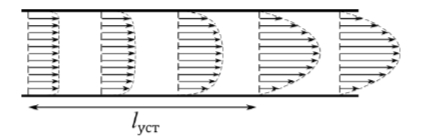
\includegraphics[width = 0.6\textwidth]{fig1.jpg}
    \caption{Формирование установившегося течения}
  \end{center}
\end{wrapfigure}
При втекании газа в трубку из большого резервуара скорости слоев вначале постоянны по всему сечению (рис. 1). По мере продвижения газа по трубке картина распределения скоростей меняется, так как сила трения о стенку тормозит прилежащие к ней слои. Характерное для ламинарного течения параболическое распределение скоростей устанавливается на некотором расстоянии $a$ от входа в трубку, которое зависит от радиуса трубки $r$ и числа Рейнольдса по формуле
\[a \approx  0,2 r \cdot Re \text{ } \text{ } \text{ } (3)\]
Градиент давления на участке формирования потока оказывается большим, чем на участке с установившимся ламинарным течением, что позволяет разделить эти участки экспериментально. Формула (3) дает возможность оценить длину участка формирования.
\section{Экспериментальная установка}
Измерения производятся на экспериментальной установке, схема которой изображена на рис. 2. Поток воздуха под давлением, несколько превышающим атмосферное (на 5-7 см вод. ст.), через газовый счетчик ГС поступает в резервуар А, к которому припаяны тонкие металлические трубки. Примерные размеры трубок указаны на рисунке (точные размеры обозначены на установке). Обе трубки на концах снабжены заглушками, не пропускающими воздух. Во время измерений заглушка открывается только на рабочей трубке; конец другой трубки должен быть плотно закрыт. Перед входом в газосчётчик поставлена U-образная трубка, наполовину заполненная водой. Она выполняет две задачи. Первая - измерение давления газа на входе в газосчётчик. Вторая - предохранение газосчётчика от выхода из строя. Дело в том, что газосчётчик устойчиво работает, если давление газа на его входе не превышает 600 мм водяного столба. Высота U-образной трубки примерно 600 мм, поэтому, когда давление на входе в счётчик превышает 600 мм водяного столба,вода из U-образной трубки выплёскивается в защитный баллон Б и, создавая шум, привлекает к себе внимание экспериментатора.

\begin{figure}[h]
\begin{center}
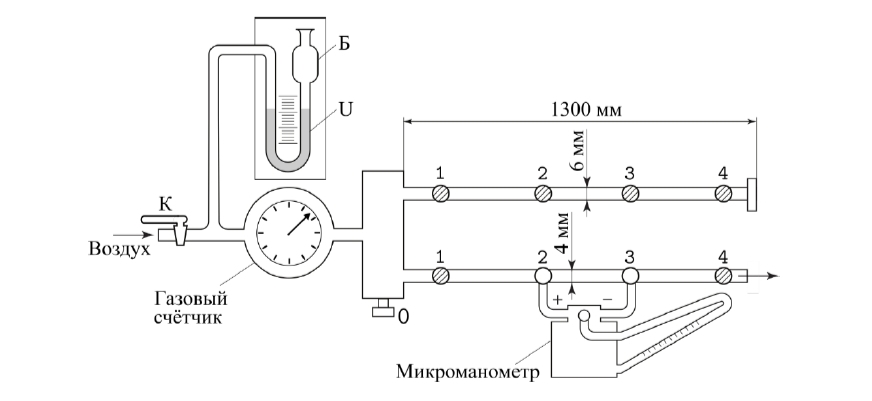
\includegraphics[width = 0.9\textwidth]{fig2.jpg}
\caption{Схема установки}
\end{center}
\end{figure}

\section{Ход работы}
Подготавливаем установку к работе: устанавливаем приборы по уровням, проверяем наличие воды в газовом счетчике по водомерному устройству, установливаем на ноль мениск микроманометра. Мы использовали три трубки разного диаметра.
\begin{center}
$d_1=3,95 \pm 0,05$ mm, $d_2=3,00 \pm 0.1$ mm, $d_3=5,05 \pm 0,05$ mm\\
\end{center}
На рис. 3 показана реальная экспериментальная установка, откуда мы можем видеть, что среди трех трубок есть две длинные и одна короткая.В двух длинных трубках есть четыре участника, а в короткой трубке есть три участника.

\begin{figure}[h]
\begin{center}
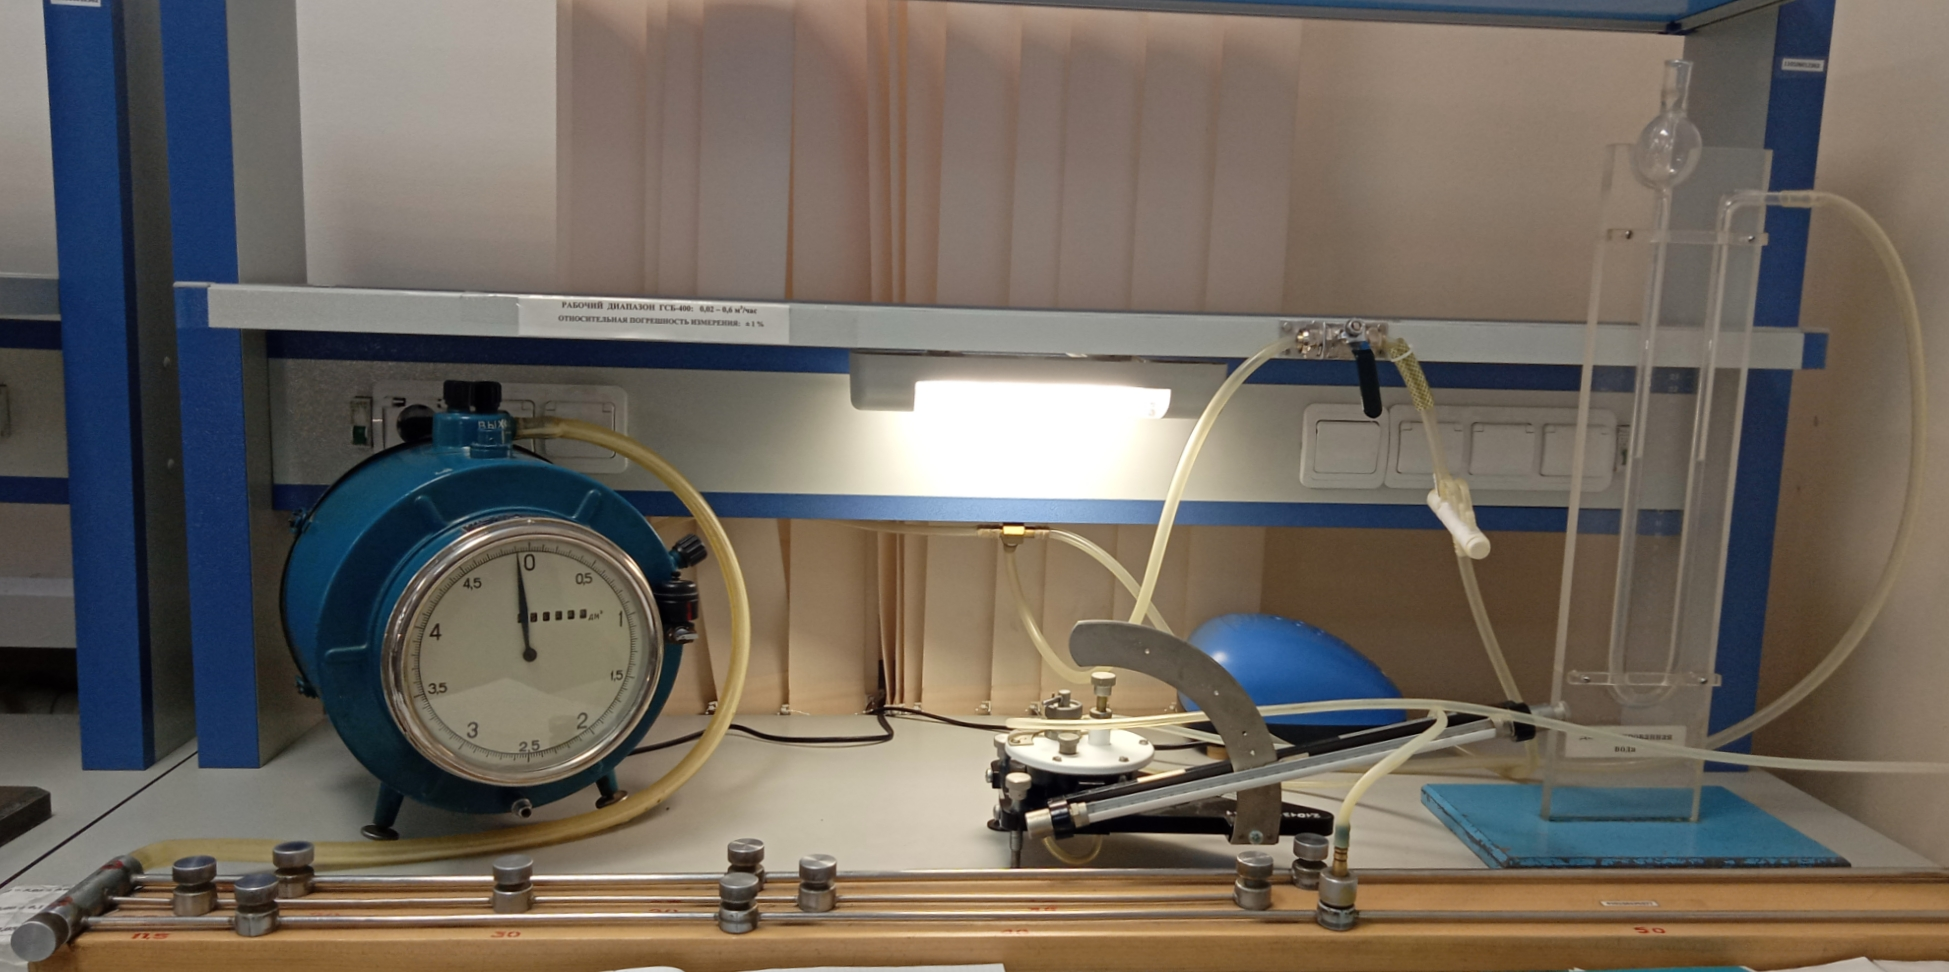
\includegraphics[width = 0.9\textwidth]{fig3.jpg}
\caption{Реальная экспериментальная установка}
\end{center}
\end{figure}
В таблице 1 b 2 ниже мы записываем различную длину участей труб.

\begin{table}[h!]
\centering
\begin{tabular}{|c|c|c|}
\hline
Участие двух длинных трубок & $l$, см & $\sigma$, мм \\ \hline
0 - 1                 & 11      & 1            \\ \hline
1 - 2                 & 30      & 1            \\ \hline
2 - 3                 & 40      & 1            \\ \hline
3 - 4                 & 50      & 1            \\ \hline
\end{tabular}
\caption{Длины участков двух длинных трубок между различными точками подключения.}
\label{tab:second_tube_parametrs}
\end{table}

\begin{table}[h!]
\centering
\begin{tabular}{|c|c|c|}
\hline
Участие одной короткой трубки & $l$, см & $\sigma$, мм \\ \hline
0 - 1                 & 6.5      & 1            \\ \hline
1 - 2                 & 20      & 1            \\ \hline
2 - 3                 & 20      & 1            \\ \hline
\end{tabular}
\caption{Длины участков одной короткой трубки между различными точками подключения.}
\label{tab:second_tube_parametrs}
\end{table}
Проведем измерение зависимости перепадов давления от расхода воздуха. Для этого будем отмерять либо 5, либо 7,5 литров воздуха, проходящих через газовый счетчик, засекая время начала и время окончания замера. Результаты занесем в таблицы.

\begin{table}[h]

	\centering
	\begin{tabular}{|c|c|c|c|c|c|c|c|c|} \hline
  $\Delta V, \, \text{л}$ &   $l,\, \text{мм}$ &     $t_1, c$ &     $t_2, c$ &     $t_3, c$ &     $t_4, c$ &     $t_5, c$&     $ Q, 10^{-3} \frac{\text{л}}{c} $ & $\Delta P, 10^{-3}\, \text{Па}$ \\\hline
 4.5 &30 &  119 & 148 & 132 &  125 & 126 & 34.62&  58.8 \\\hline
 5 &  48 &  83 &  84 &  82 &  86 &  85 &   59.52& 94.08 \\\hline
 5 &  63 &  63 &  64 &  65 &  62 &  63 &   78.86& 123.48 \\\hline
 5 &  70 &  58 &  58 &  58 &  59 &  58 &   85.91& 137.2   \\\hline
 5 &  108 & 49 &  51 &  51 &  52 &  50 &   98.81& 211.68   \\\hline
 5 &  146 & 44 &  44 &  44 &  45 &  45 &   112.61& 286.16    \\\hline
  
\end{tabular}
		\caption{Измерения на трубке $d_1$ с расстоянием $50$ см}
\end{table}


Из графика (рис.4) мы видим, что поток был ламинарным до 85.91, а затем со $88 \pm 2$ он переходит в турбулентный.\\
Коэффициент угла наклона графика: $k = 1.597 \frac{\text{Па} \cdot c}{\text{mm}^3}$

Искомая вязкость:
\[
	\eta = \frac{\pi r^4 k}{8 l} = 0.0191 \text{Па} \cdot \text{c}
\]
Из графика видно, что ламинарный режим переходит в турбулентный на значениях $Q \approx 88 \cdot 10^{-6} \frac{\text{м}^3}{c}$
Посчитаем число Рейнольдса:
\[
	Re = \frac{vr\rho}{\eta} = 	\frac{Q \rho}{\pi r \eta} \approx  750
\]
\begin{figure}[h]
\center
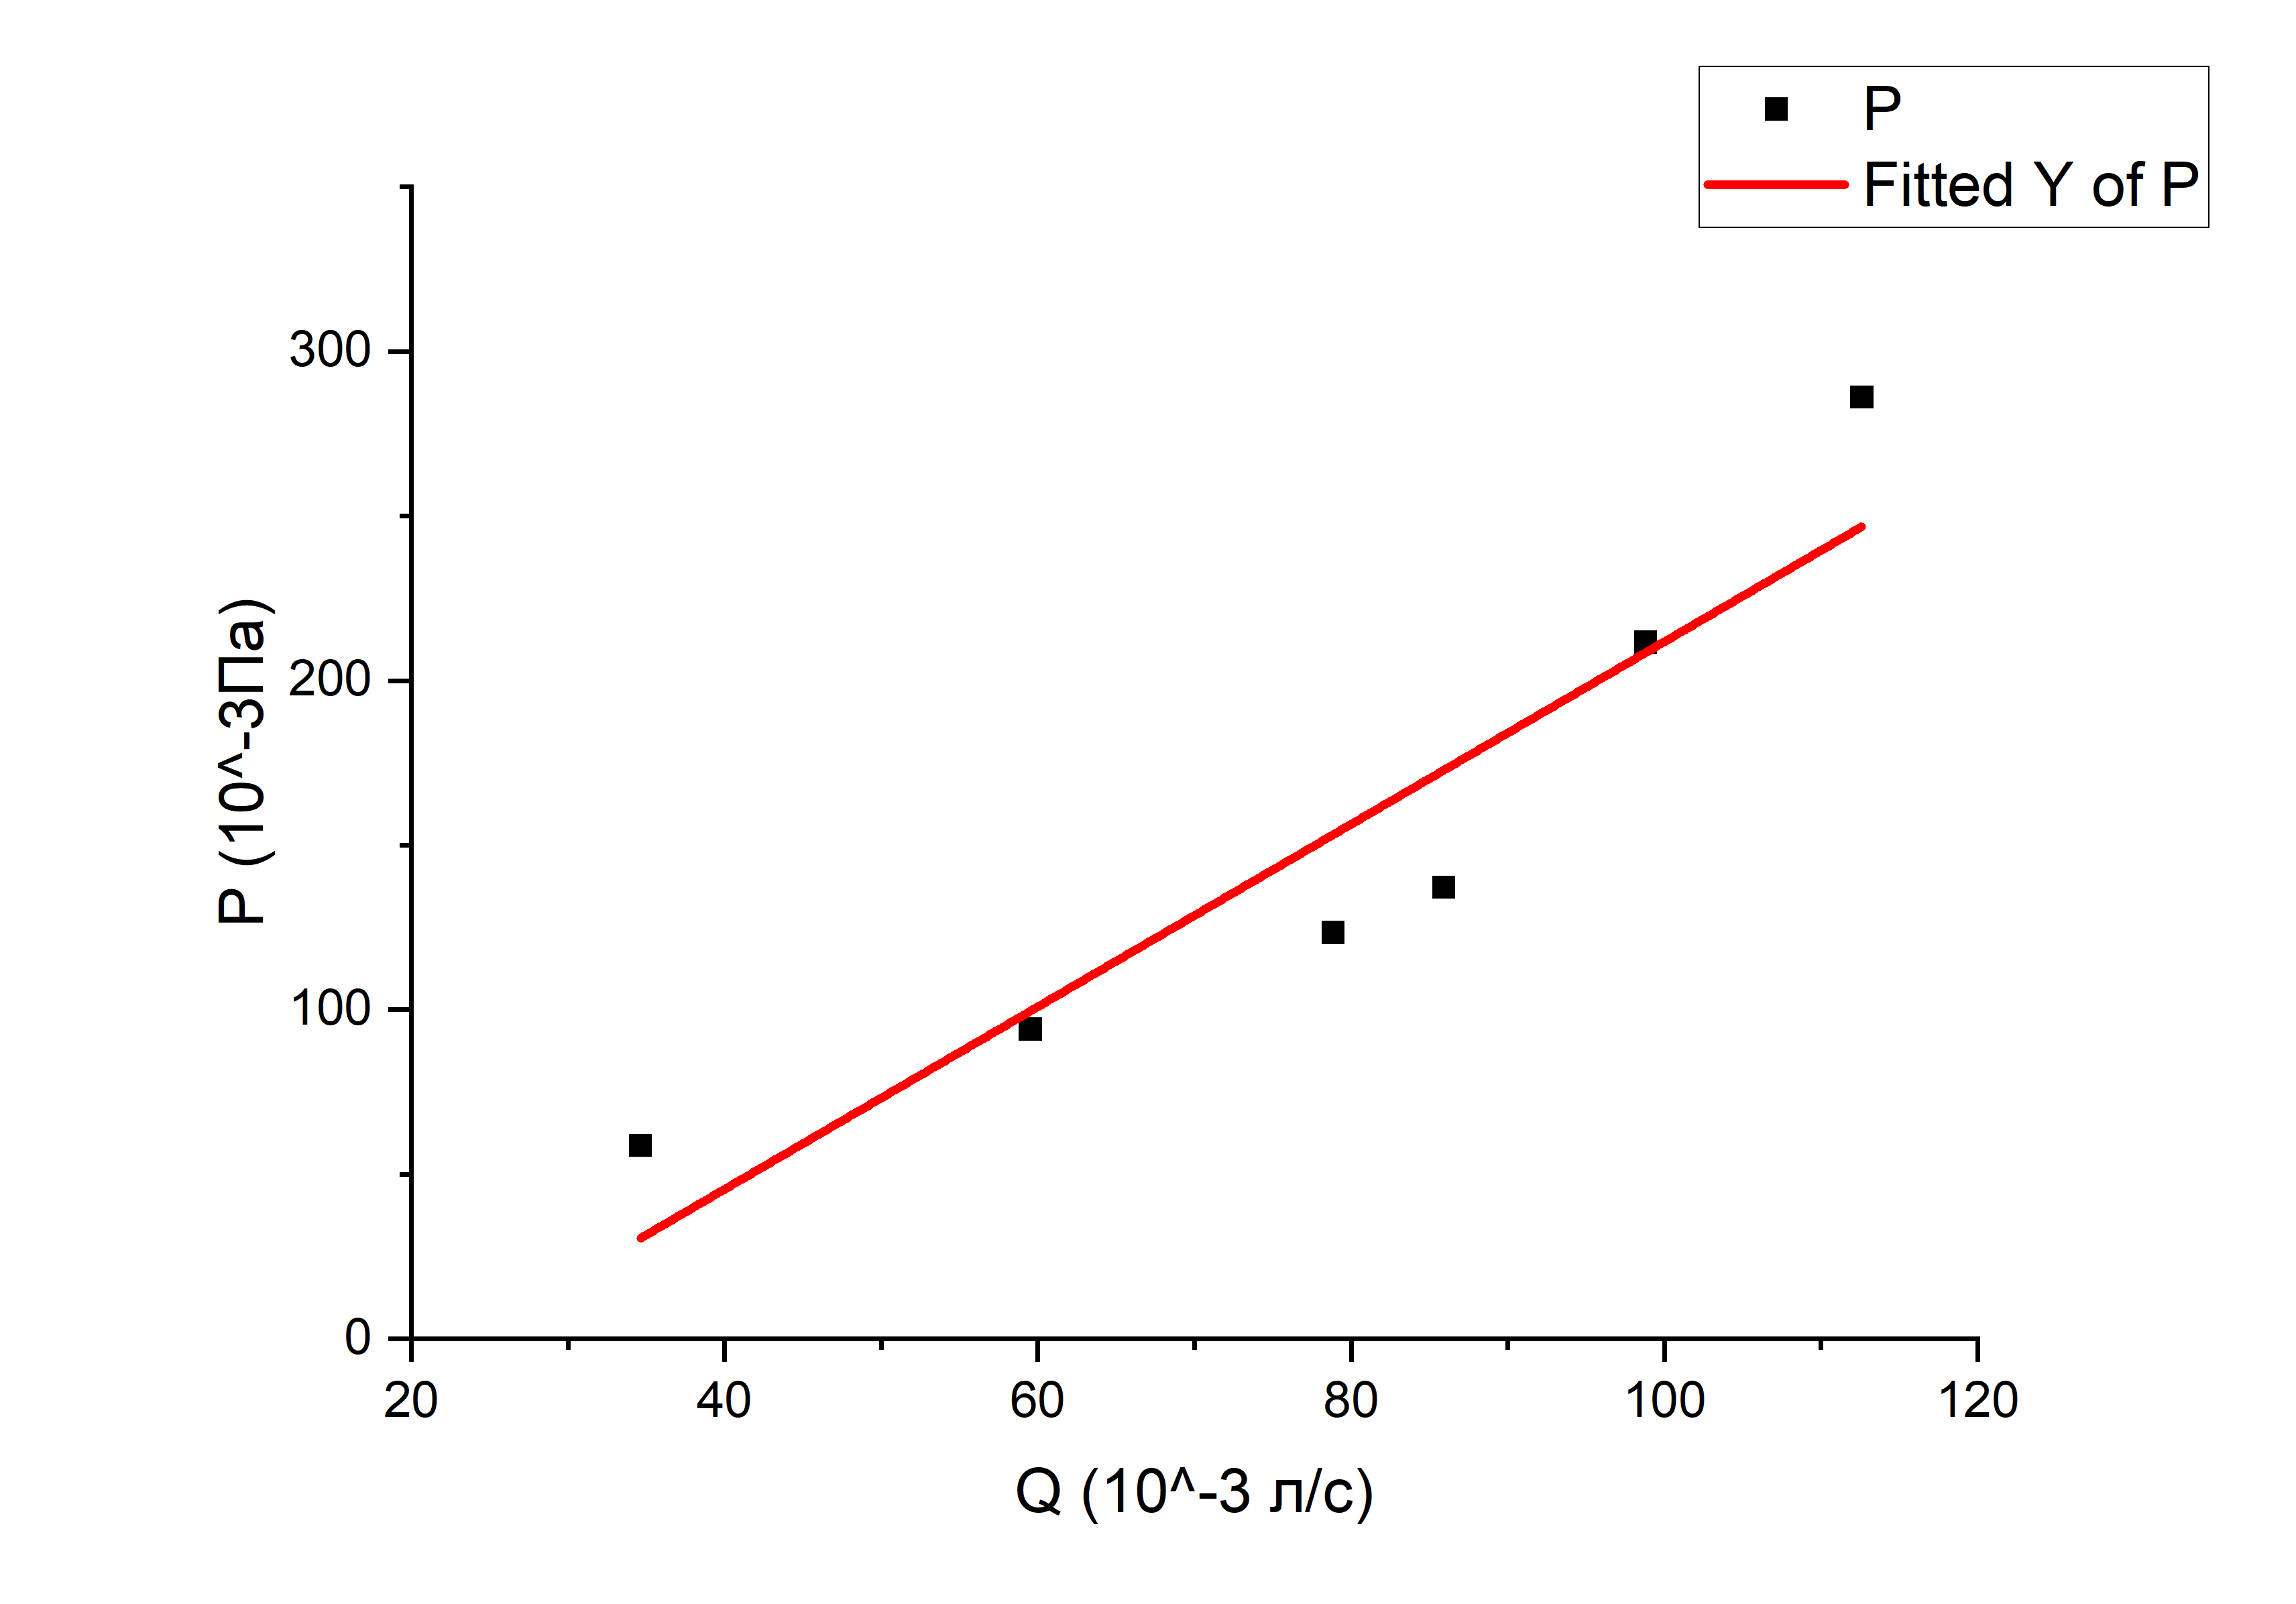
\includegraphics[scale=0.4]{labphoto8.png}

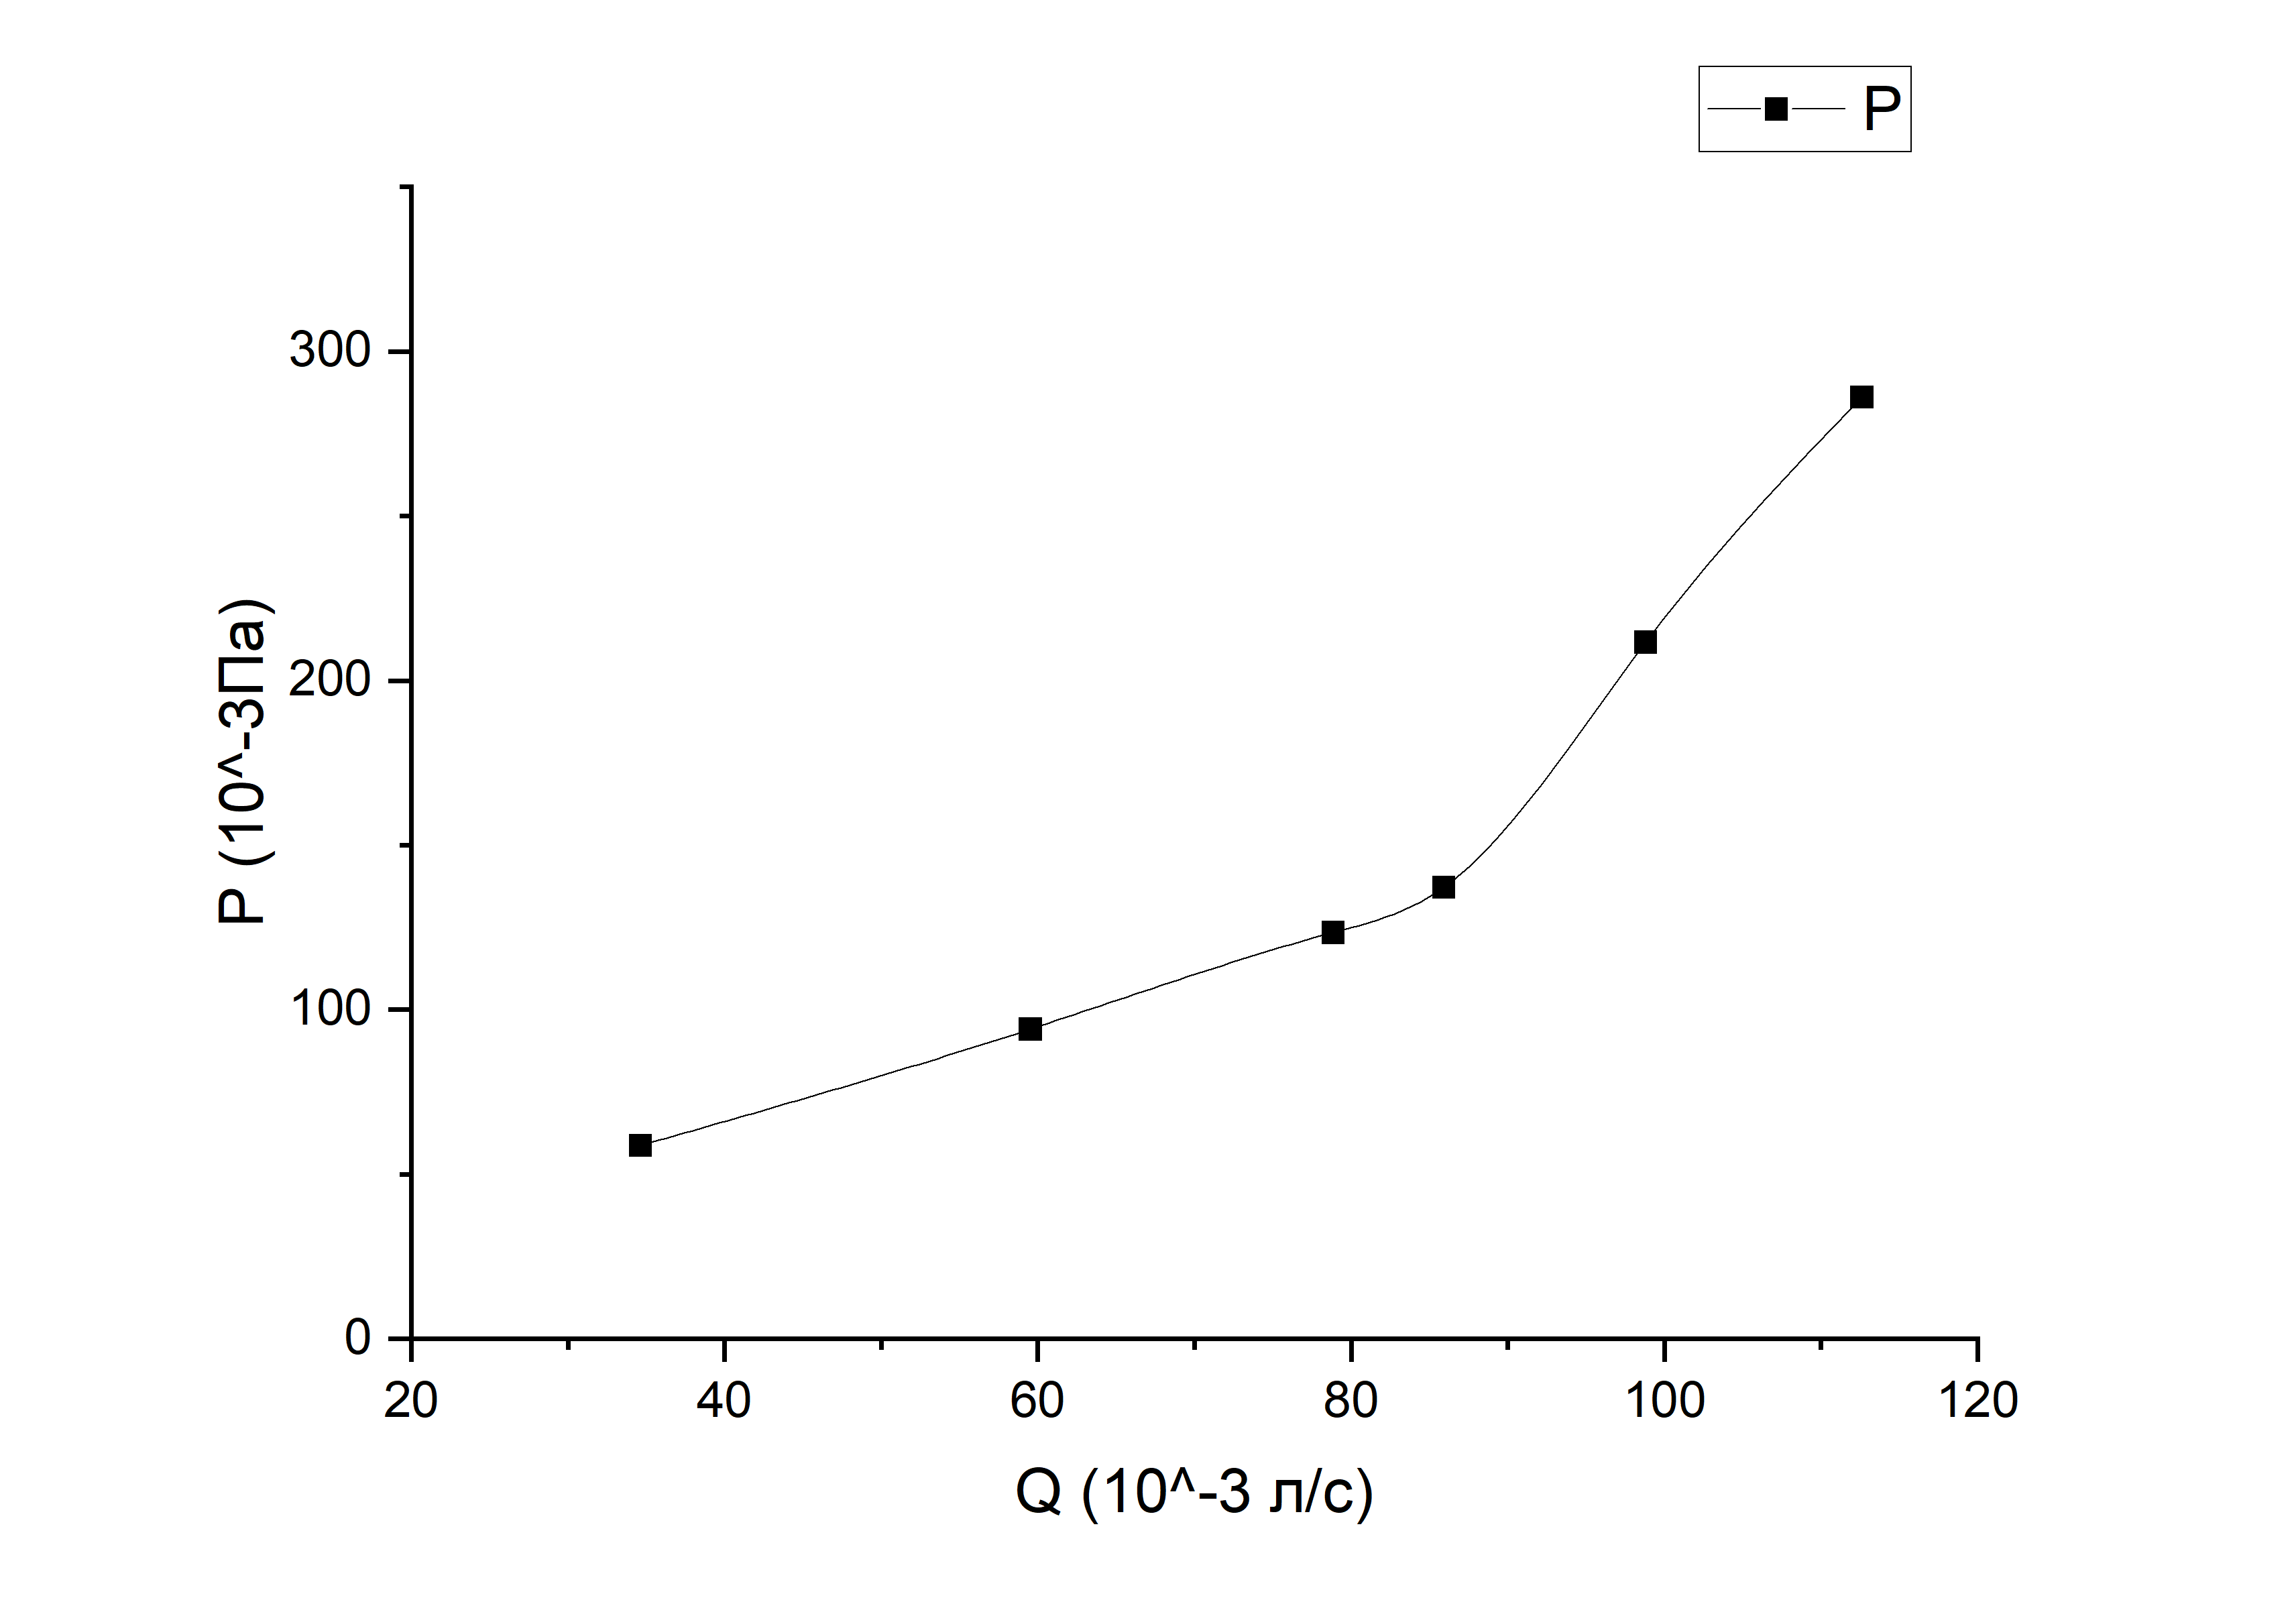
\includegraphics[scale=0.4]{labphoto9.png}
\caption{Spline connected $Q$ vs $\Delta P$ в трубке $d_1$ с расстоянием 50 см}
\end{figure}
\newpage

Теперь мы сменили трубку на $d_3$. Его радиус больше, чем у $d_1$.  В приведенной ниже таблице приведены данные о расходе и разности давлений для трубы $d_3$.
\begin{table}[h]

	\centering
	\begin{tabular}{|c|c|c|c|c|c|c|c|c|} \hline
 $\Delta V, \, \text{л}$ &   $l,\, \text{мм}$ &     $t_1, c$ &     $t_2, c$ &     $t_3, c$ &     $t_4, c$ &     $t_5, c$&     $ Q, 10^{-3} \frac{\text{л}}{c} $ & $\Delta P, 10^{-3}\, \text{Па}$ \\\hline
5 &  32 &  43 & 44 & 44 &  43 & 41 & 115.61   &  62.72 \\\hline
5 &  63 &  32 & 32 &  31 &  33 &  32 & 154.32 & 123.48 \\\hline
5 &  92 &  27 &  27 &  28 &  27 &  28 &   185.19& 180.32 \\\hline
5 &  121 &  23 &  23 &  24 &  25 &  23 &  215.51 & 237.16   \\\hline
5 &  149 & 20 &  21 &  21 &  19 &  22 &   240.38& 292.04   \\\hline
5 &  165 & 19 &  19 &  20 &  19 &  20 &   257.73& 323.4    \\\hline
 \end{tabular}
		\caption{Измерения на трубке $d_3$ с расстоянием $50$ см}
\end{table}

\begin{figure}[h]
\begin{center}
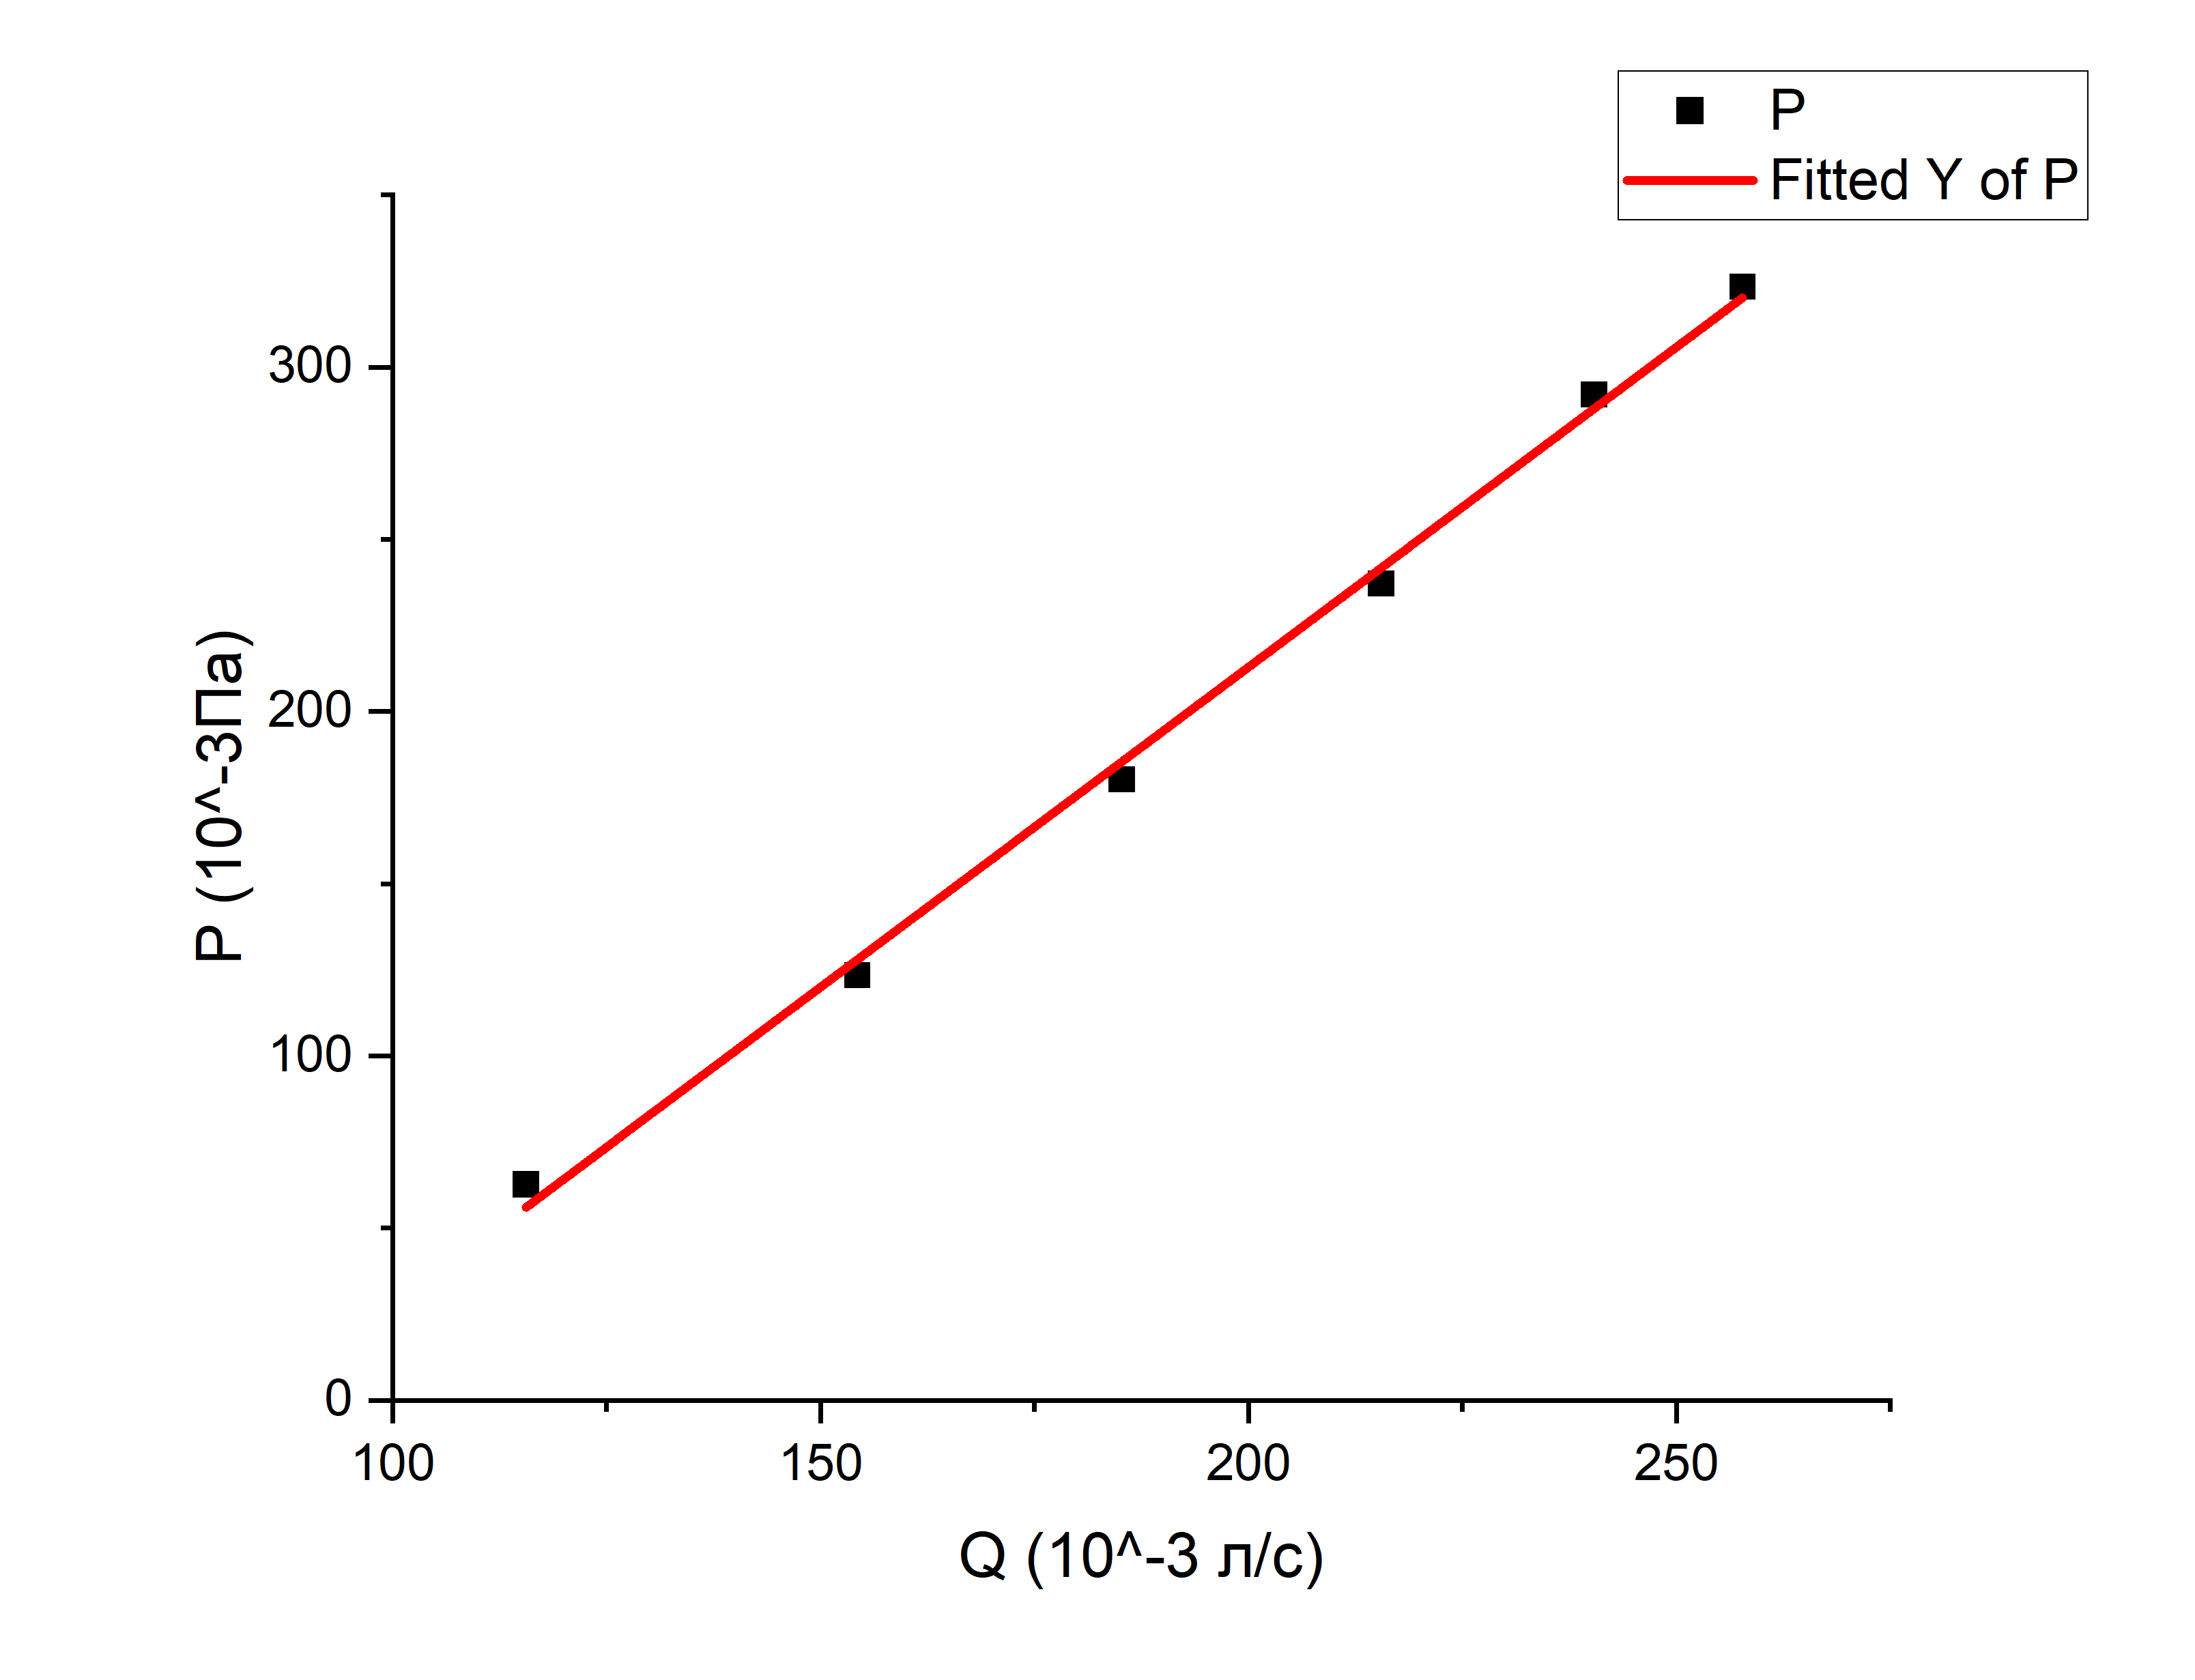
\includegraphics[width = 0.8\textwidth]{labphoto6.png}
\caption{$Q$ vs $\Delta P$ в трубке $d_3$ с расстоянием 50 см}
\end{center}
\end{figure}

\newpage На этом графике мы видим, что поток линейный, это означает, что во всем нашем эксперименте с этой трубкой поток был ламинарным. Поскольку скорость потока Q и давление P больше, чем раньше, то в этом случае длина ламинарного потока больше, чем была раньше, и тогда начнется турбулентность, которую мы не могли видеть на графике.\\
\linebreak
 Теперь мы поддерживаем постоянный поток и смотрим, как меняется давление с увеличением длины. Мы используем все сечения наших трех разных труб и строим их на одном графике, чтобы понять разницу из-за их диаметра.
\newpage
\begin{table}
 \begin{tabular}{|c|c|c|c|c|c|c|c|c|}
\hline
\multicolumn{3}{|c|}{$d = (5,05 \pm 0,05)$ мм} & \multicolumn{3}{c|}{$d = (3,95 \pm 0,05)$, мм} & \multicolumn{3}{c|}{$d = (3,00 \pm 0,1)$, мм} \\ \hline
$l$, cm, & $\Delta P$, mm & $\Delta P, 10^{-3}\, \text{Па}$,& $l$, cm,& $\Delta P$, mm, & $\Delta P, \text{Па}$ & $l$, cm,& $\Delta P$, mm & $\Delta P,\text{Па}$ \\ \hline
131.5 & 241 & 472.36 & 131.5 & 237 & 464.52 & 46.5 & 139 & 272.44 \\ \hline
81.5 & 169 & 331.24 & 81.5 & 174 & 341.04 & 26.5 & 88 & 172.48 \\ \hline
41.5 & 92 & 180.32 & 41.5 & 124 & 243.04 & 6.5 & 42 & 82.32 \\ \hline
11.5 & 56 & 109.76 & 11.5 & 45 & 88.2 & & & \\ \hline
\end{tabular}
\caption{Параметры при постоянном расходе}
\end{table}

\begin{figure}[h!]
	\begin{center}
		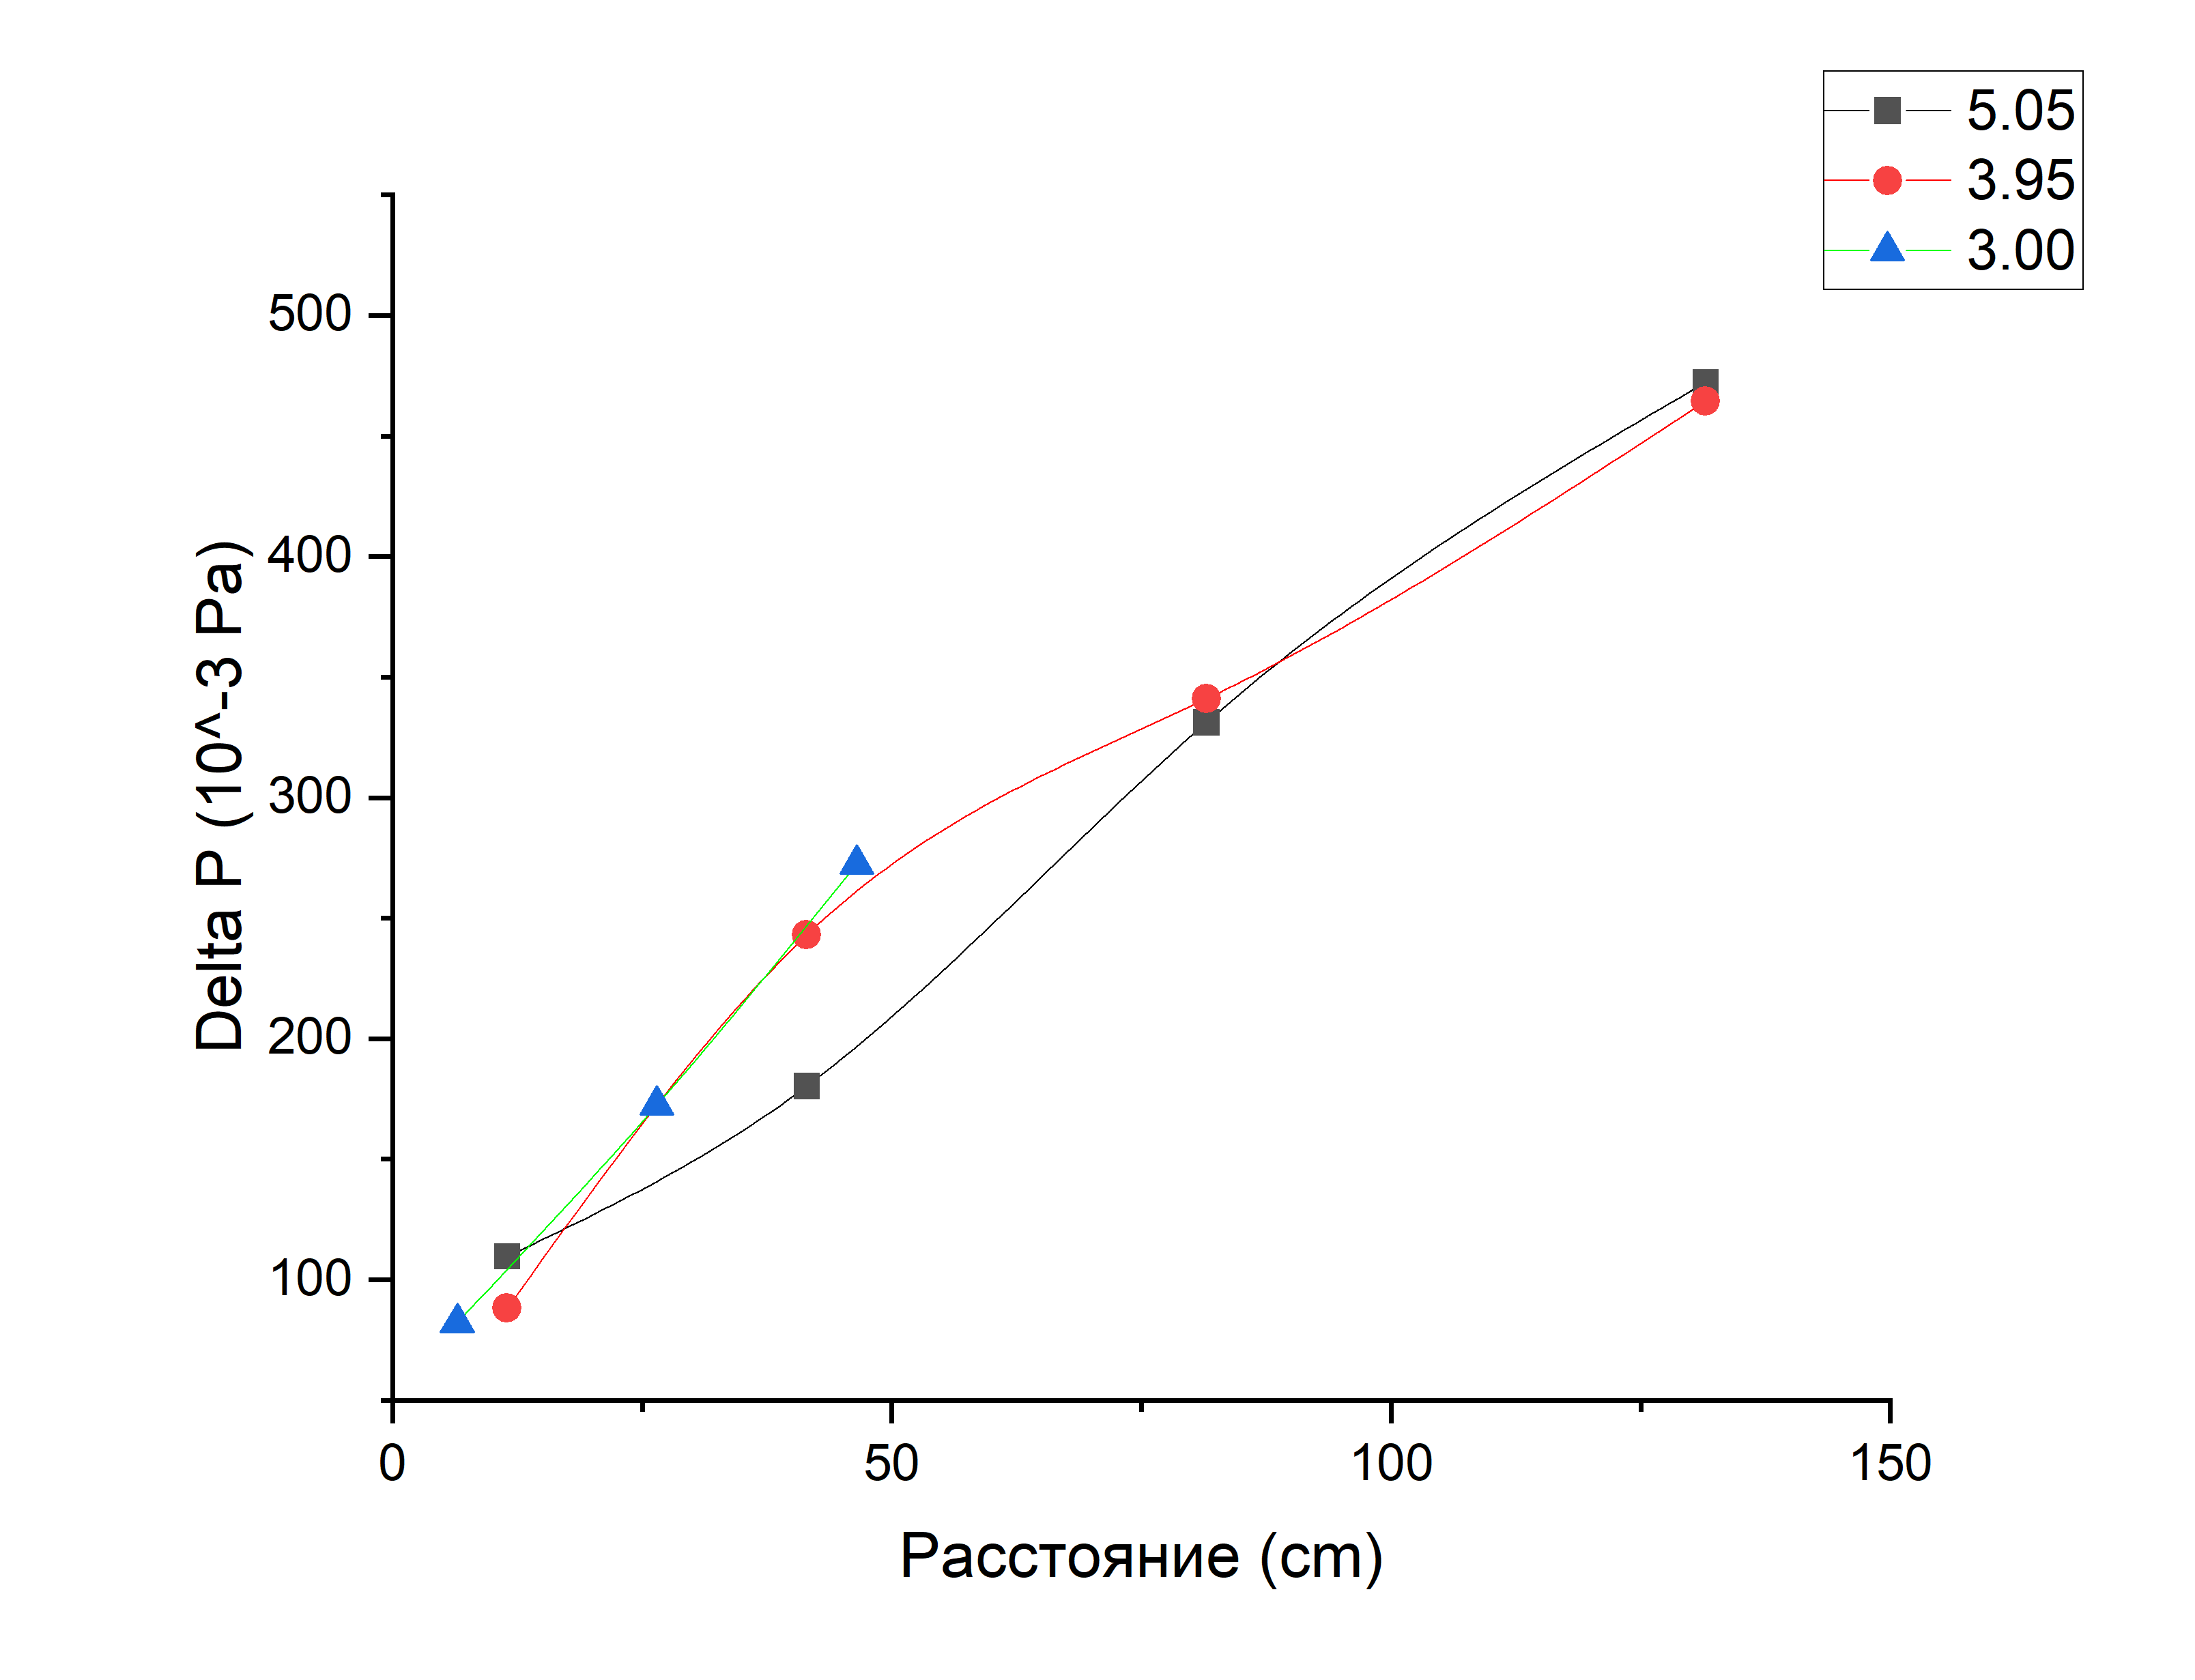
\includegraphics[width = 0.85\textwidth]{labphoto11}
		\caption{графики зависимости перепада давления от расстояния до начала трубки}
	\end{center}
\end{figure}

\section{Вывод}
Из теории мы знаем, что ламинарный поток станет турбулентным, когда число Рейнольдса станет 1000. В нашем первом эксперименте мы получили число Рейнольдса приблизительно 750, поэтому на нашем графике мы видим, что максимальный ламинарный поток, а затем переходящий в турбулентный,когда скорость потока более 88 л /с. \\
\linebreak В следующем эксперименте (рис.5) с большим диаметром трубы мы видим, что поток намного выше, и поскольку вязкость пропорциональна четвертой степени радиуса, поэтому по мере увеличения радиуса вязкость также должна увеличиваться, что означает, что мы должны получить меньшее число Рейнольдса, чем раньше. Из чего следует вывод, что должен получиться полный ламинарный поток в этой жировой трубке.
\begin{figure}[h]
\center
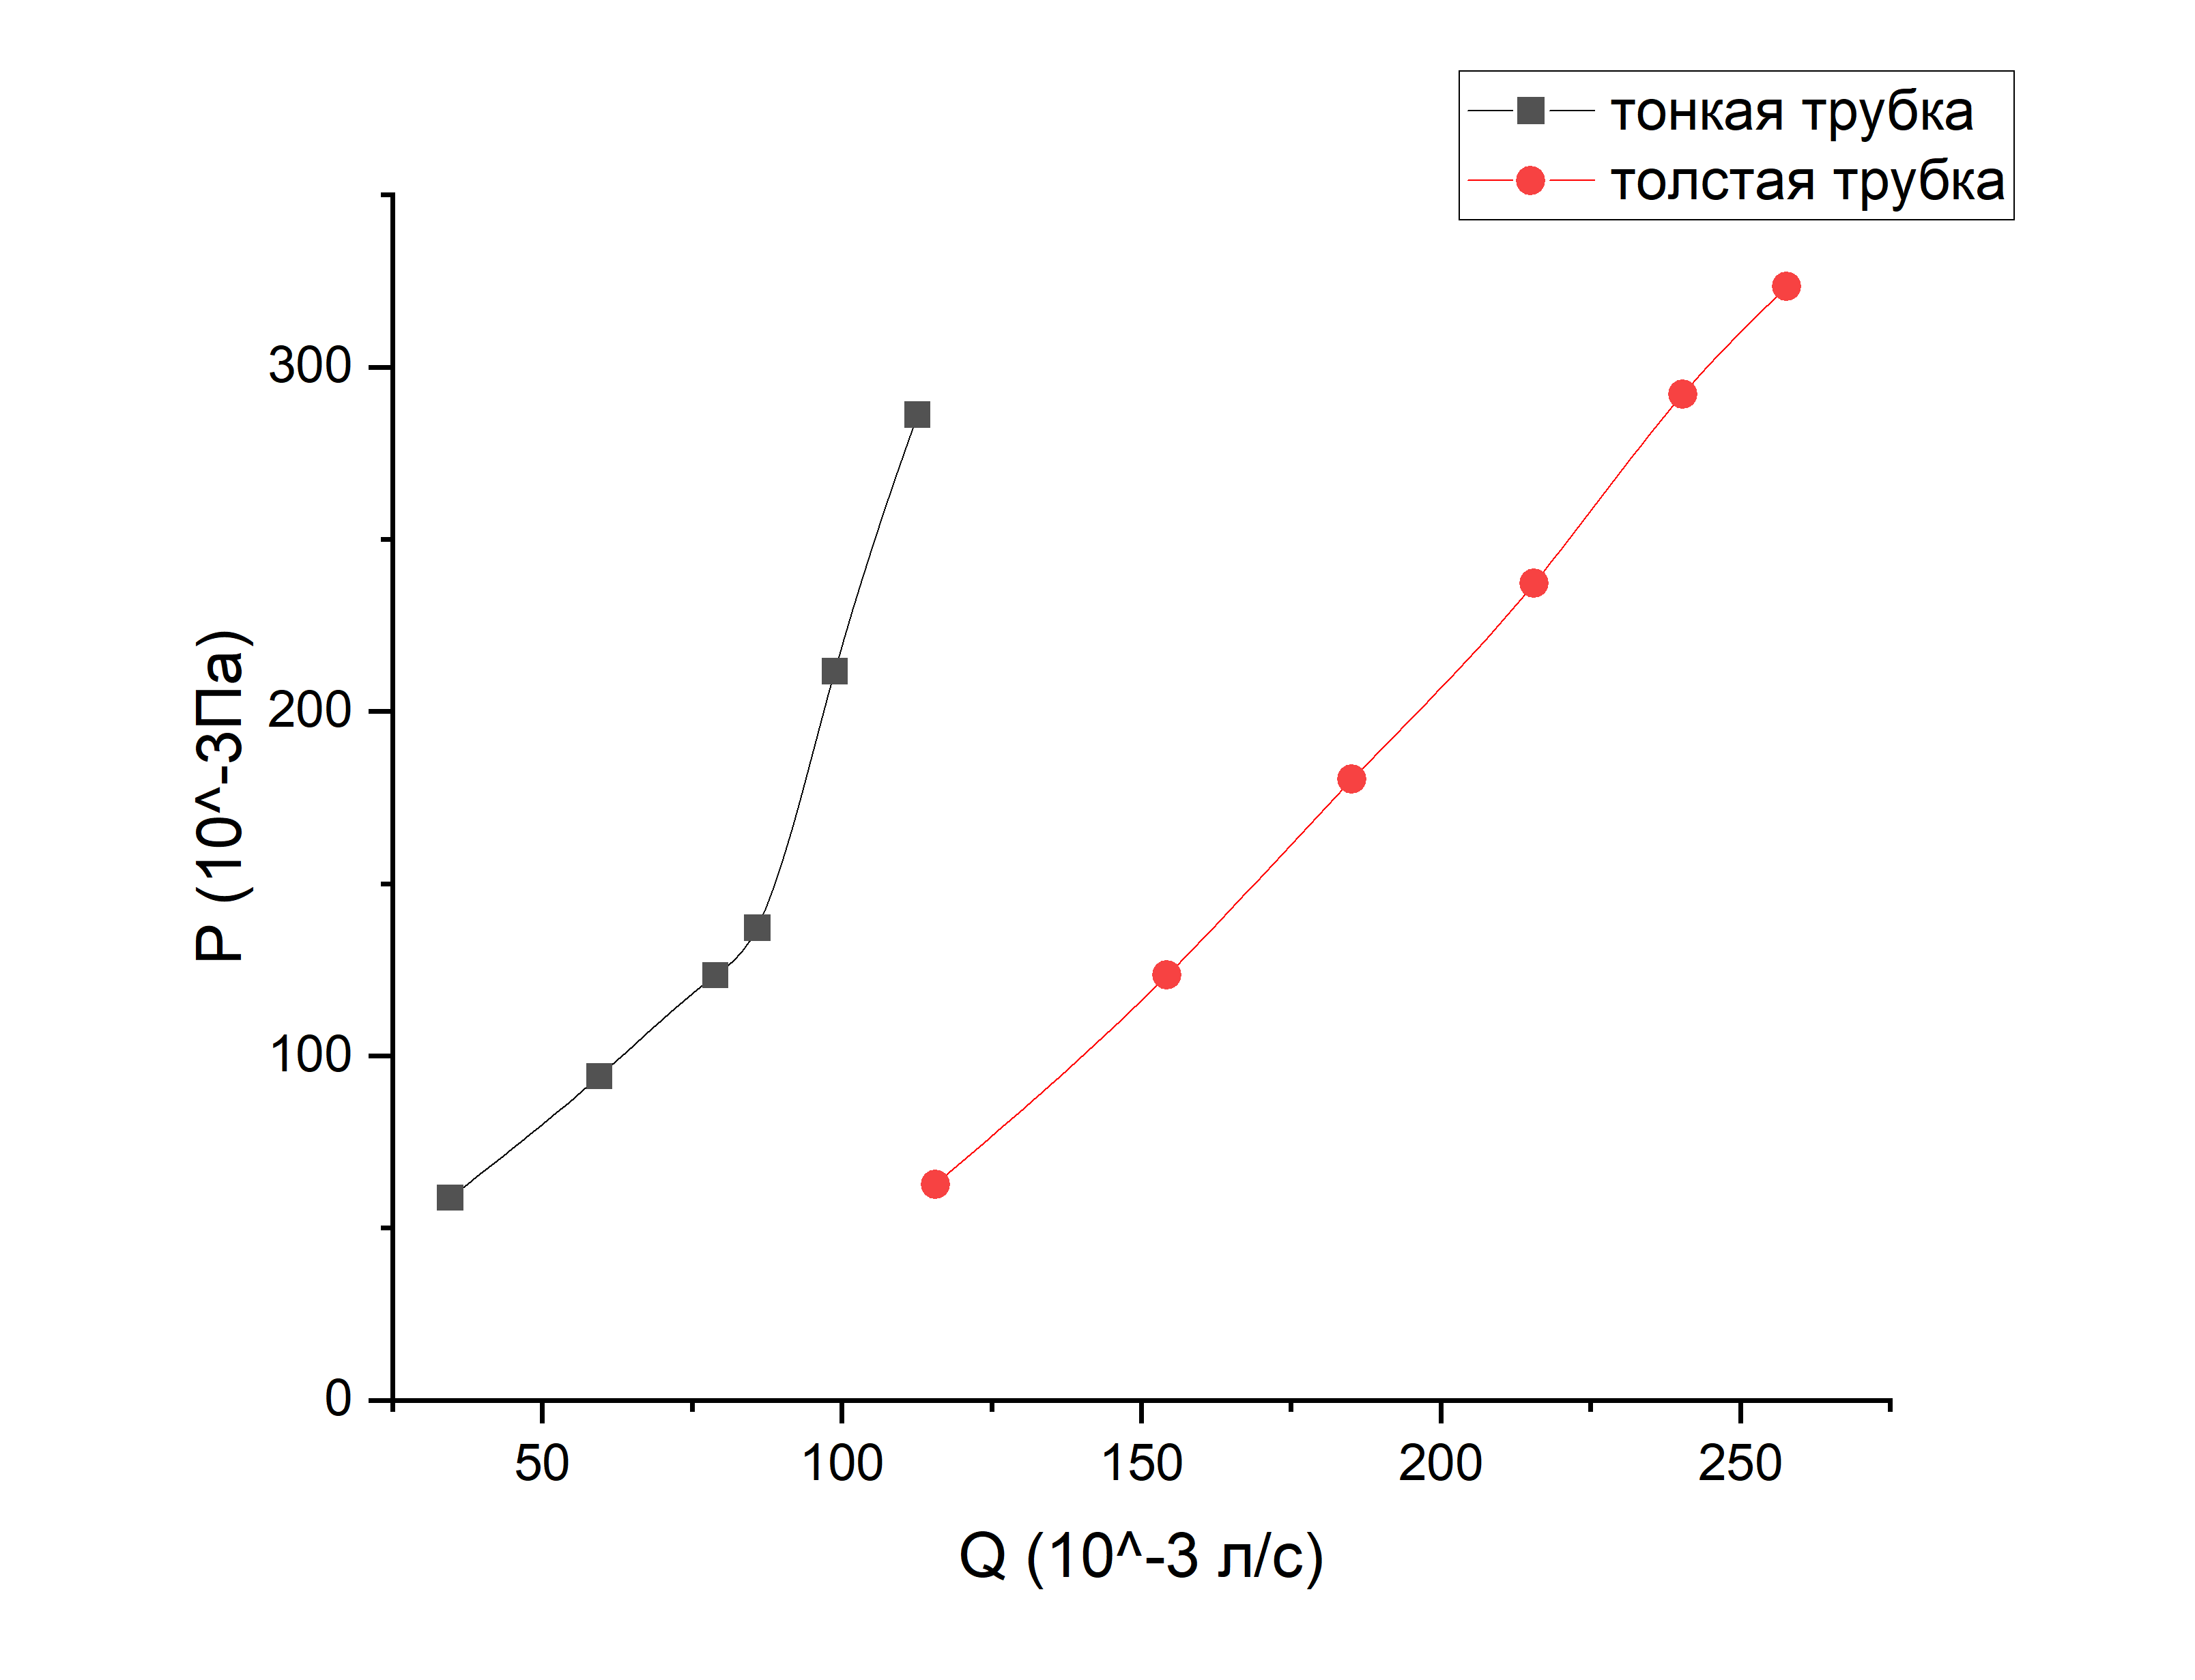
\includegraphics[scale=0.4]{labphoto12.png}
\caption{Сравнение двух экспериментов с толстой и тонкой трубкой}
\end{figure}

\newpage В последней части нашего эксперимента мы поддерживали постоянный поток, поэтому градиент давления изменился для трех разных труб. К сожалению, мы по ошибке открыли пробку на расстоянии 11,5 мм, поэтому во время измерения значения манометра мы записали немного неправильные данные, которые показывают на графике(рис.6), что скорость изменения давления в трубке диаметром 3,95 мм пересекает линию трубки диаметром 5,05 мм, чего никогда не должно быть.





\end{document}